% !TEX root = ../thesis-example.tex
%
\chapter{Conclusion}
\label{sec:conclusion}

\begin{flushright}{\slshape    
If people never did silly things\\
nothing intelligent would ever get done.} \\ \medskip
--- Ludwig Wittgenstein~\cite{Luckhardt:1979}
\end{flushright}

\bigskip

In this thesis, we have adopted a `physicist' approach to the study of a system
that traditionally belonged to the realm of social sciences: the city. We have
tried to show that simple approaches allow to better understand
these complex systems. Although simple models with a few variables cannot
reproduce all the properties and behaviours of the observed phenomena, they
allow us to uncover the dominant mechanisms that are responsible for their most
salient features. Does it mean that our approach is the only valid approach?
Probably not. It is useful? Certainly, as it structures
our knowledge and sets a solid basis for future investigations.\\

% Make sure everything is in the past tense
In the first part, we have reviewed the evolution of the concept of
polycentricity in the literature, and the methods used to identify and count the
number of centers. Doing so, we provided evidence for the increasing number of
activity centers with population size, a phenomenon we called `polycentric
transition'. We then proposed an out-of-equibrium, stochastic model of
city growth that reproduces the empirical regularity, and explains the
transition with the increasing levels of congestion as cities get larger. This
model is a substantial improvement over the models presented in the Economics
literature: it makes predictions that are supported by data, and allows to
identify the phenomenon responsible for the observed phenomenon. 

In the second part, we further use the model to give a prediction for the
scaling exponent of the total distance commuted daily, the total length of the
road network, the total delay due to congestion, the quantity of
CO\textsubscript{2} emitted, and the surface area with the population size of
cities. We successfully test these predictions with data gathered for US urban
areas.

In a third part, we focus on the quantitative description of the patterns of
residential segregation. For the first time in the quantitative literature, we
propose an explicit definition of segregation as a deviation from a random
distribution of individuals across the urban space. This definition provides a
unifying theoretical framework in which segregation can be empirically
characterised. We propose a measure of interaction between the different
categories. Building on the information about the attraction and repulsion
between categories, we are further able to propose a definition of classes that
is quantitative and unambiguous. The framework also allows us to identify the
neighbourhoods where the different classes concentrate, and characterise their
properties and spatial arrangement. Finally, we revisit the traditional
dichotomy between poor city centers and rich suburbs and provide a measure that
is adapted to anisotropic, polycentric cities. 

In the fourth and last part, we briefly reviewed the results we have obtained in
the study of spatial networks. We first presented a quantitative method to
classify cities based on their street patterns, which we applied to a set of
$131$ cities across the world. Then, we introduced an iterative model for the
growth of spatial networks that is based on cost-benefit considerations. The
model exhibits interesting features: a crossover between the Minimum Spanning
Tree and the star graph, with an intermediate regime characterised by the
emergence of spatial hierarchy. Finally, we proposed a general coarse-grained
approach -- based on a
cost-benefit analysis -- that accounts for the scaling properties of the main
quantities characterizing railway and subway networks (the number of stations, the total
length, and the ridership) with the substrate's population, area and wealth.
We showed that the length, number of stations and ridership of
subways and rail networks can be estimated knowing the area, population and
wealth of the underlying region. These predictions are in good agreement with
data gathered for about $140$ subway systems and more than $50$ railway networks in the
world.\\ 

The field is still in its infancy compared to more mature sciences, but there
are very good reasons to hope for the convergence of knowledge and methods into
a new discipline. Into what we may call -- following Michael Batty -- a Science of
Cities. It is difficult at this stage to say what this Science will look like,
and what kind of results it can pretend to achieve. Nevertheless, it is tempting to
compare the current state of the field to the study of planetary motions
before Isaac Newton's \emph{Philosophi\ae Naturalis Principia Mathematica}, or
the study of electromagnetism before James Clerk Maxwell's \emph{A Dynamical
Theory of the Electromagnetic Field}; a set of stylized facts and empirical laws
that are yet to be unified in a coherent theory. 

This is not to say that one should look for a unifying set of equations, or that
laws about urban system will have the same permanence as those describing
natural phenomena. No two theories are alike -- even in Physics. But we believe
that the underlying methodological principles have a universal character.
Nothing can go fundamentally wrong if data are the ultimate judge of the
validity of the products of our theoretical endeavours.



\section{Lessons learned}
\label{sec:what_the_past_3_years_have_brought}

The last $3$ years have taught me lessons that go beyond simple scientific
knowledge.

\subsection{Thinking the city}
\label{sub:thinking_the_city}

A first lesson, painstakingly learned during this thesis is that \emph{thinking} the
city is as important as \emph{measuring} the city, or \emph{modeling} the city.
Concepts guide us and tell us what to measure, what to model. In the same way
measures and model can tell us what to think. It would be very naive to
believe that scientific enquiries are fueled by the sole discussion between
measures and models. In fact, many studies are based upon an hypothesis, a
pattern that the author has seen and whose existence she is trying to prove on a
quantitative basis. 

It is also certainly true that the most difficult and important problems are
conceptual in nature.  It is impossible to define a city quantitatively a city
before you have formed---with words, possibly drawings---a conceptual picture of
what a city is.  It is impossible to study segregation before you have logically
clarified what one means by segregation. However quantitative, an investigation
built upon weak conceptual foundations is unlikely to go anywhere, or to say
anything substantial. On the other hand, when the thoughts have settled and the
question is clear, one can quickly make a substantial contribution. In this
sense, qualitative and quantitative investigations are not incompatible: they
are really two sides of the same coin.\\


\subsection{Disciplinary borders}
\label{sub:disciplinary_borders}


The topics I had the chance to tackle during these 3 years of PhD were very
diverse. In retrospect, this was a real chance. This pushed me to peruse a wide
literature that encompassed many different disciplines. What I found striking
while perusing articles and books is the tendency of the different communities to
ignore one another. 

The problem, however, is not to blame on individuals. While there may be
deliberate omissions here and there, authors are generally willing to cite the
appropriate literature when they are aware of its existence. The issue, I
believe, is institutional. It stems from the academic organisation of Science,
and the existence of disciplinary borders.

But do disciplinary borders still mean anything? While there is an undeniable
historical justification to the existence of disciplines, do they still make
sense, scientifically speaking? Should the path-dependency in the evolution of
the man-made, academic classification of sciences dictate what research avenues
are worth being pursued today? At a time when some topics -- including cities
-- get an increasingly multi-disciplinary attention, these questions are worth
asking. Science is fueled by ignorance and questions, not knowledge. It may therefore be
time to organise communities around common questions, rather than (overlapping)
corpora of knowledge.


\section{If I had to write a second thesis (Future directions)}
\label{sec:limitations}

What would I write about -- or at least try to -- if I had to start my
thesis all over again? This is another way of saying: what are the next steps?
Many clues can be found in the various parts of the thesis. Indeed, I have tried
to explicit the limitations of the empirical methods and models presented. In
these remarks lie many potential avenues for future research. In the following,
I will present some other ideas that sprung over the last $3$ years.\\

I would probably start with the basics, with the single noun that was most often
printed in these pages: Cities~\footnote{\emph{Not} verified on data.}. It is
indeed uncomfortable -- to say the least -- that our most fundamental object,
the city, is ill-defined, and that most empirical studies possibly rely on a definition
that is not suited to the investigation they undertake.  This lack of serious
definition compromises the comparison between cities of different countries, or
at different points in time. I am, of course,
not the first person to acknowledge this empirical shortcoming. In fact, it has
been a long-time worry of geographers who have been trying to produce harmonised
database for a long time~\cite{Pumain:2015}. Yet, we still lack of an
unambiguous, theoretically grounded definition of what a city is. And this is
problematic, since statistical institutes' results are based on what is believed
to be the best definition of the city at a time. Which in turns influences the
research on cities. If we want to exhibit robust empirical results, compare the
results obtained in different countries, we therefore need to start worrying
about the definition of the system we are studying. We need to know \emph{what}
cities we are talking about.\\

\begin{figure}
    \centering
    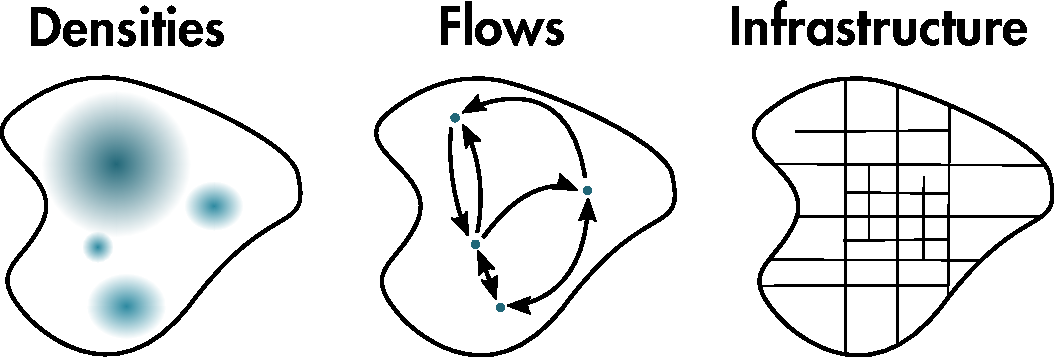
\includegraphics[width=1\textwidth]{gfx/chapter-intro/intra-urban.pdf}
    \caption{{\bf Intra-urban organisation.} Cities are first and foremost defined by
    the concentration of populations and various activities. The fact that
residences and activities have different locations is responsible for the
existence of flows of people, goods, etc. across the urban space. These flows
occur on appropriate infrastructure.\label{fig:intra_urban}}
\end{figure}


Once the boundaries are defined, we can start studying the way objects are
scattered within them. By objects, I mean buildings, roads, and first and
foremost people. The way we traditionally study the repartition of objects in
space is through the study of densities. But density profiles are too
complicated to comprehend for our brains, especially when cities get large. So
complicated, that an entire sub-field is dedicated to their study: urban
form~\cite{Tsai:2005,Schwarz:2010,LeNechet:2015}.
Authors attempt to solve this problem by providing simple measures 
that extract a single number from the profile. A single number is however too
simple to be able to describe accurately complex spatial distributions. What we need
is a meso-scale representation, somewhere between the micro-scale picture (the
density profile itself) and the macro-scale picture (a single number to
summarize the density profile). Hopefully, because `centers' are themselves a
mesoscopic structure, their definition should emerge naturally from such a
representation.\\


Once one is able to provide an accurate description of density profiles, the
possibilities start to diverge. An obvious worry, when one has a picture of the
city's population at different times of the day, is the way these profile
transform one into another. This is linked to commuting --but not only,
commuting representing only $20\%$ of total travels in the
US~\cite{FHWA-PL-11-022}-- and the study of congestion of networks. 

We could first try to explicit the link between the urban form (typically the
residential and employment densities) and mobility
patterns~\cite{Ma:2006,Chowdhury:2013}.  For instance, we could wonder: what
proportion of commuting flows is due to the spatial mismatch between jobs and
residences? 

A futher worry linked to commuting is that of congestion:
understanding how traffic jams are formed, how they propagate and devise
strategies to mitigate them, either by influencing the transportation
infrastructure, the spatial repartition of residences and employment, or the
behaviour of people themselves.  This is far from being a recent worry, but
there is room for new approaches that leverage the knowledge we have about
network and phase transition in physics. A first step in this direction has been
made by the authors of~\cite{Li:2015}, but there is surely more to be understood
and discovered.  

Modeling congestion also implies understanding the individual behaviour of
people when they are moving from a point to another in cities. Altough most
research nowadays assume that people choose the shortest (time or distance)
path, GPS data now provide overwhelming evidence that this is not the
case~\cite{Manley:2015}. So, while there is a clear need to understand the mesoscopic
picture (how congestion spread), there is also is a critical need to understand
the microscopic picture (how people behave).\\


So far we have talked about the movement induced by the spatial mismatch between
residential areas and activity areas. One might also want to study the
characteristics of the spatial repartition of people. Inhabitants of cities are
not just a combination of a latitude and a longitude, a point on a map. Like you
and me, they are characterised by different qualities, some of which are
measurable: say their income, their education level, their ethnicity, etc. A
natural question, that has interested sociologist and geographers, is to wonder
whether people's residence is independent of these characteristics, or whether
these characteristics have an influence on the spatial repartition of
individuals.  

In this thesis, we provided a rigorous method to study the patterns of
segregation in the presence of multiple income categories. The method is far
more general, however. It could be used to study the concentration of any
category (be it ethnic categories, or certain business types, etc.)
in certain regions of the urban space, and quantify the resulting spatial pattern. As a
matter of fact, more work is needed to be able to identify the topology and
geometry of these distributions. The problem is very close to the description of
density pattern described above.

The definition of neighbourhoods (again, a mesoscopic structure) is also not
completely satisfactory. Often, it relies on non-overlapping census boundaries
that were drawn to maximise the intra-neighbourhood homogeneity and maximise the
inter-neighbourhoods heterogeneity. Although this may be useful for political
institutions to target the most segregated regions of the city, this does not
account for how segregation is witnessed by individuals, at an individual level.
This has recently been questioned in the Sociology literature, and there has
recently been new attempts to define neighbourhoods based on social ties~\cite{Hipp:2012}.\\

There are many more ideas that would deserve to be explored, many more topics
that are worthy of attention. I hope the years to come will give me the opportunity
to address some of them. But not now; this thesis has to stop somewhere.  
